% Template for Cogsci submission with R Markdown

% Stuff changed from original Markdown PLOS Template
\documentclass[10pt, letterpaper]{article}

\usepackage{cogsci}
\usepackage{pslatex}
\usepackage{float}
\usepackage{caption}

% amsmath package, useful for mathematical formulas
\usepackage{amsmath}

% amssymb package, useful for mathematical symbols
\usepackage{amssymb}

% hyperref package, useful for hyperlinks
\usepackage{hyperref}

% graphicx package, useful for including eps and pdf graphics
% include graphics with the command \includegraphics
\usepackage{graphicx}

% Sweave(-like)
\usepackage{fancyvrb}
\DefineVerbatimEnvironment{Sinput}{Verbatim}{fontshape=sl}
\DefineVerbatimEnvironment{Soutput}{Verbatim}{}
\DefineVerbatimEnvironment{Scode}{Verbatim}{fontshape=sl}
\newenvironment{Schunk}{}{}
\DefineVerbatimEnvironment{Code}{Verbatim}{}
\DefineVerbatimEnvironment{CodeInput}{Verbatim}{fontshape=sl}
\DefineVerbatimEnvironment{CodeOutput}{Verbatim}{}
\newenvironment{CodeChunk}{}{}

% cite package, to clean up citations in the main text. Do not remove.
\usepackage{cite}

\usepackage{color}

% Use doublespacing - comment out for single spacing
%\usepackage{setspace}
%\doublespacing


% % Text layout
% \topmargin 0.0cm
% \oddsidemargin 0.5cm
% \evensidemargin 0.5cm
% \textwidth 16cm
% \textheight 21cm

\title{Word Learning as Network Growth: A Cross-linguistic Analysis}

\usepackage[subtle]{savetrees}

\author{{\large \bf Abdellah Fourtassi} \\ \texttt{afourtas@stanford.edu} \\ Department of Psychology \\ Stanford University \And {\large \bf Yuan Bian} \\ \texttt{ybian.uiuc@gmail.com} \\ Department of Psychology \\ University of Illinois \And {\large \bf Michael C. Frank} \\ \texttt{mcfrank@stanford.edu} \\ Department of Psychology \\ Stanford University}

\begin{document}

\maketitle

\begin{abstract}
Children tend to produce words earlier when they are connected to a
variety of other words along both the phonological and semantic
dimensions. Though this connectivity effect has been extensively
documented, little is known about the underlying developmental
mechanism. One view suggests that learning is primarily driven by a
network growth model where highly connected words in the child's early
lexicon attract similar words. Another view suggests that learning is
driven by highly connected words in the external learning environment
instead of highly connected words in the early internal lexicon. The
present study tests both scenarios systematically in both the
phonological and semantic domains, and across 8 languages. We show that
external connectivity in the learning environment drives growth in both
the semantic and the phonological networks, and that this pattern is
consistent cross-linguistically. The findings suggest a word learning
mechanism where children harness their statistical learning abilities to
(indirectly) detect and learn highly connected words in the learning
environment.

\textbf{Keywords:}
semantic network, phonological network, network growth, mechanism of
word learning
\end{abstract}

\section{Introduction}\label{introduction}

How do children acquire words? An important step consists in mapping a
phonological form (e.g.~the sound ``cat'') to a semantic referent (the
concept CAT). A large body of work has been devoted to explore the
mechanism of this mapping (Quine, 1960; Markman, 1990; Smith and Yu,
2008). However, words do not exist in a vacuum; they are organized into
a strcuture based on both semantic and phonological similarity
principles (e.g., Collins \& Loftus, 1975; Luce \& Pisoni, 1998). A more
accurate understanding of word learning should account not only for how
sounds are mapped to meanings, but also for how sound similarity and
meaning similarity may influence the process of aqusition.

We know that similarity affect word recognition in both adults and
children. For example, exposure to a word such as ``cat'' influences
subsequent recognition of phonologically and smantically similar words
like ``cab'' and ``dog'' (Goldinger, Luce \& Pisoni, 1989; McNamara,
2006; Arias-Trejo \& Plunkett, 2010; Mani \& Plunkett, 2011).

Crucially, similarity influences not only the recognition of know words,
but also the learning of novel words. For example, Swingley \& Aslin
(2007) showed that infants found it more challenging to learn the
meaning of a novel word such as ``tog'' (which is similar a the familiar
word ``dog'') than to learn the meaning of a word such as ``shang''
(which is not similar to any words children knew). When learning two
novel words, Stager and Werker (1997) found that infatns were more
likely to succeed when these words were phonologically distant (e.g.,
``lif''/``neem''), than when they were phonologcially simialr
(``bin/''din``). Besides, children learn the semantic relationship among
newly learned words spontaneousely (Wojcik \& Saffran, 2013), and they
prioritize the acquisition of words that are distinct in the semantic
space (Engelthaler \& Hills, 2017).

That said, previous experimental work has studied the effect of
phonological and semantic similarity separately. Some studied the
mechanism of word learning using a toy lexicon where only the
phonological similarity varied (e.g., Stager and Werker, 1997), and
others studied the learning of a toy lexicon where only the semantic
similarity varied (e.g., Wojcik \& Saffran, 2013). However, children
acquire a lexicon which is more richly structured than these special
cases. In particular, as reviewed abvove, the end-state lexicon involves
variability along both the phonological and semantic domains. Thus, to
have a deeper understanding of word acquisition in the real world, it is
crucial to study how learners acquire a lexicon that simulates this
bi-dimensional variation.

One could imagine two learning scenarios. On the first one, children's
learning, at least in some challenging situations, is primarily
determined by one dimension (Sloutsky \& Napolitano, 2003; Colavita et
al. 1975). For example, it is possible that similar sounding words are
confusable and hard to learn regardless of their semantic similarity.
Vice-versa, similar meanings might be challenging to learn regardless of
the phonological similarity of their forms. On the second scenario,
learners combine cues from both dimensions to optimize their learning
(Fourtassi and Frank, 2018; Ernst \& Banks, 2002). Thus, confusability
that may arise from high similarity along one dimension can be mitigated
via higher distance from the other dimension. In this study, we explore
these hypothesis, bla bla

A second goal of this work is to investigate how the learning mechanism
develops over the life span. According to one hypothesis, adults use
qualitatively distinct learning mechanisms than children, due, for
example, to maturational factors. To illustrate, in the experimental
setting used in Stager and Werker (1997), children's difficulty with
learning similar sounding words--despite their ability to perceptually
differentiate them--might be attributed to their inferior working
memory, hindering their ability to attend simultaneously to the sound
contrast and the meanings. A second hypothesis proposes that learners
use fundamentally similar mechanisms across the life span, and that the
difference might be one of degree, not kind. For example, though they
have vastly greater working memory capacity, adults show patterns of
word processing and learning which parallel results obtained with
children in Stager and Werker's study (White et al. 2013; Pajak et al.
2016). Here we explore

Talk a bit about what we do

\section{Experiment 1}\label{experiment-1}

Children were trained to learn the association between pairs of
nonesense words (e.g., ``lif''/``neem'') and pairs of objects (e.g., two
flowers). After training, children performed a series of two-alternative
forced choices. In each testing trial, one of the two sounds is uttered
(e.g., ``lif'') and participants choose the corresponding object from
the two alternatives (e.g., flower 1 or flower 2). Each child learned an
artificial lexicon where both the pairs of sounds and the pairs of
objects can be similar or different. Our predictions were as follows. If
the sound and meaning interact in word learning, then the pair of words
that differ on both the meaning and sound levels should be the easiest
to learn, followed by the pairs of words that are different on one
level, but similar on another level. Finally, the pair of words that are
similar on both levels should be the most difficult to learn.

\subsection{Methods}\label{methods}

\subsubsection{Participants}\label{participants}

We planned to recruit a sample of 60 children ages 4-5 years from the
Bing Nursery School on Stanford University's campus. So far, we
collected data from N=47 children (mean age= months, F=). An additional
28 children participated but were removed from analyses because they
were not above chance on the catch trials (as specified in the
pre-registration).

\subsubsection{Stimuli}\label{stimuli}

The sound stimuli were generated using the MBROLA Speech Synthesizer
(Cite) using an American English voice. We generated two similar sound
pairs (``aka''/``ama'' and ``ada''/``aba'') and two different sound
pairs (``lif''/``neem'' and ``zem''/``doof''). We generated a addtional
pair (``nak''/``veep'') which we used in the catch trial (see
Procedure). As for the objects used as semantic referents, we used the
Dynamic Categories Stimuli (Cite) which allowed us to generate objects
in four different categories: ``tree'', ``bird'', ``bug'', and ``fish''
(plus the additional category ``flower'' for the catch trial). These
categories are supposed to be naturally occuring kinds that might be
seen on an alien planet. In each category, we generated instances that
varied in their similarity by manipuating a continuous property
controling features of the category's shape. This property was the head
fatness for the category ``bug'', the body strech for ``bird'', the tail
size relative to the body fatness for ``fish'', the width of the trunk
for ``tree'', and finally center size for ``flower''. All these
continous properties varied on a scale from 0 to 1. We generated
``similar'' and ``different'' objects' pairs (whithin each category) by
setting the values of this properties to 0 and 0.5, and to 0 and 1,
respectively. Examples of the resuting pairs are shown in Figure XX.

\subsubsection{Design}\label{design}

The experiment consisted of 4 conditions which consisted, each, of a
pair of sounds-objects associations. These conditions were constructed
by crossing the sound's degree of similarity with the object's degree of
similarity leading to a 2x2 factorial design. Besides the 4 conditions,
we also tested participants on a fifth catch condition which was similar
to the previous ones. It involved different sounds and different
objects, and it was used only to select participant who were able to
follow the instructions and show minimal learning (not at chance level).

\subsubsection{Procedure}\label{procedure}

Children were asked if they would be willing to play a game on a tablet
with the experimenter and were informed that they could stop playing at
any time. The experimenter explained that the game consisted in learning
some words spoken in an alien planet. The experiment began with two
simple examples (not included in the analysis), and in these examples
children were given feedback from the experimenter so as to make sure
they correctly understood the structure of the task. After the
introduction and examples, children were tested in a sequence of five
conditions: the four experimental conditions plus the catch condition.
In each condition, participants saw a first block of four exposure
trials followed by four testing trials, and a second block of two
exposure trials (for memory refreshment) follwoed by an additional four
testing trials.

In the exposure trials, children saw two objects associated with their
corresponding sounds. We presented the first object on the left side of
the tablet's screen simultaneously with the corresponding sound. The
second sound-object association followed on the other side of the screen
after 500ms. For both objects, visual stimuli were present for the
duration of the sound clip (∼800ms). In the testing trials, children saw
both objects simultaneousely and heard only one sound. They completed
the trial by selecting which of the two objects corresponded to the
sound. They responded by touching one of the pictures on the tablet.

The object-sound pairings were randomized across participants, as was
the order of the conditions (except for the catch condition which was
always placed in the middle of the testing sequence). We also randomized
the on-screen position (left vs.~right) of the two pictures on each
testing trial. The experiment can be views online using this link XX.

\subsubsection{Results}\label{results}

\begin{CodeChunk}
\begin{figure}[H]

{\centering 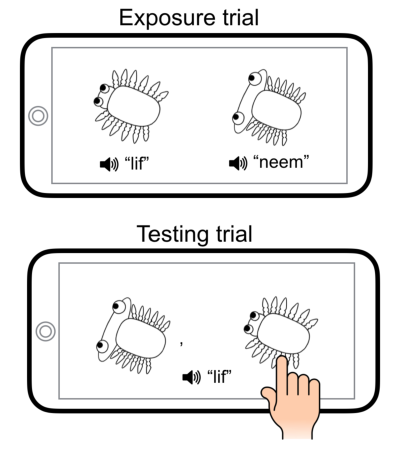
\includegraphics{figs/growth-1} 

}

\caption{\label{fig:growth}Illustration of the growth scenarios. Filled circles (I1-I4) represent known words (internal), and empty circles (E1 and E2) represent words that have not been learned yet (external). Black lines represent links that are relevant in each growth scenario, and gray lines represent links that are irrelevant. For PAT, the utility of a candidate, external node is the average degree (i.e., number of links) of the internal nodes that it would attach to. Thus, according to PAT, the node E1 is more likely to enter the lexicon first. For PAC, the utility of a candidate node is its degree in the entire network. According to PAC, the node E2 is more likely to enter the lexicon first.}\label{fig:growth}
\end{figure}
\end{CodeChunk}

Studies that investigate lexical network growth have focused on semantic
networks using English data (Hills, Maouene, Riordan, \& Smith, 2010;
Hills, Maouene, Maouene, Sheya, \& Smith, 2009; Steyvers \& Tenenbaum,
2005). The novelty of the current study is threefold: First, it
investigates whether phonological networks, like semantic networks, grow
by PAC, or if they rather grow by PAT. Second, it provides a systematic
comparison of both network growth scenarios in the phonological and the
semantic domains and assesses their relative contribution to the
learning process. Third, it tests the generality of the findings across
eight languages.

\begin{CodeChunk}
\begin{figure*}[h]

{\centering 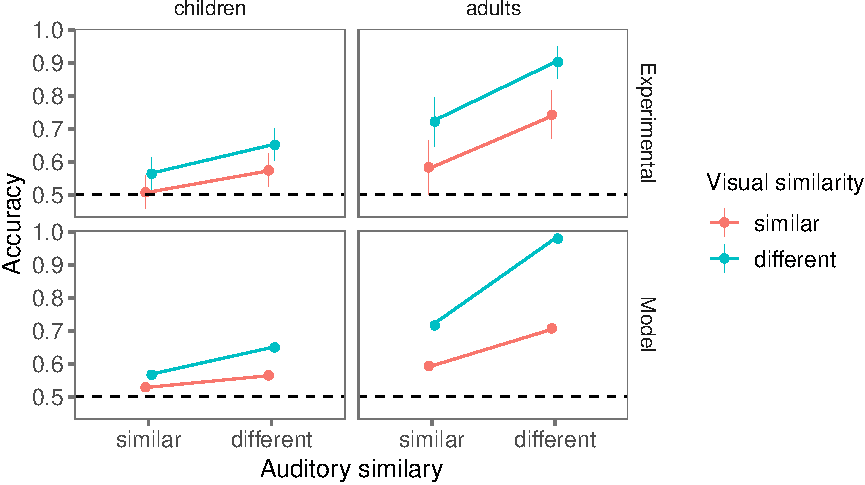
\includegraphics{figs/all_data-1} 

}

\caption{\label{fig:data_all}Age of acquisition in the global network as predicted by the degree in this network. Results are shown in each language for phonological and semantic networks. Each point is a word, with lines indicating linear model fits.}\label{fig:all_data}
\end{figure*}
\end{CodeChunk}

\begin{CodeChunk}
\begin{figure*}[h]

{\centering 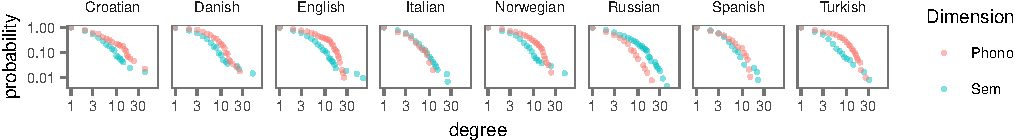
\includegraphics{figs/degree_distribution-1} 

}

\caption{\label{fig:degree_distribution}Log-log plot of the cumulative degree distribution function for the global phonological and semantic networks across languages. A perfect power-law distribution should appear as a straight line in this graph.}\label{fig:degree_distribution}
\end{figure*}
\end{CodeChunk}

\section{Networks}\label{networks}

\subsection{Data}\label{data}

We used data from Wordbank (Frank, Braginsky, Yurovsky, \& Marchman,
2017), an open repository aggregating cross-linguistic language
developmental data of the MacArthur-Bates Communicative Development
Inventory (CDI), a parent report vocabulary checklist. Parent report is
a reliable and valid measure of children's vocabulary that allows for
the cost-effective collection of datasets large enough to test
network-based models of acquisition (Fenson et al., 1994). We used the
\emph{Words and Sentences} version of the CDI which contains the
productive vocabulary of toddlers (age varied between 16 to 36 months).
Following previous studies (Hills et al., 2009; Storkel, 2009), we
restricted our analysis to nouns. We defined the age of acquisition of a
given word by the month at which this word was produced by at least 50\%
of children (J. C. Goodman, Dale, \& Li, 2008), and we excluded nouns
that have not been learned (according to this criterion) by the last
month for which we have CDI data.

We obtained these nouns in eight languages: Croatian, Danish, English,
Italian, Norwegian, Russian, Spanish, and Turkish. We used the subset of
nouns that had entries in the Florida Association Norms (see below).
Since these norms are available only in English, we used the
hand-checked translation equivalents provided by Braginsky, Yurovsky,
Marchman, \& Frank (2016), allowing us to use the English association
norms across languages. Table \ref{tab:stats} gives an overview of the
data used. Translation equivalents were originally constructed for a
subset of words appearing on the toddler CDI form, and so not all words
are currently available. Note, however, that all languages have at least
60\% of nouns translated.

\begin{table}[H]
\centering
\begin{tabular}{rlrrr}
  \hline
 & language & total & translated & normed \\ 
  \hline
1 & Croatian & 253 & 177 & 170 \\ 
  2 & Danish & 295 & 198 & 187 \\ 
  3 & English & 296 & 296 & 274 \\ 
  4 & Italian & 311 & 203 & 194 \\ 
  5 & Norwegian & 305 & 193 & 186 \\ 
  6 & Russian & 311 & 311 & 285 \\ 
  7 & Spanish & 240 & 173 & 163 \\ 
  8 & Turkish & 293 & 175 & 164 \\ 
   \hline
\end{tabular}
\caption{\label{tab:stats}Total number of nouns produced by toddlers in the CDI (left). We included in our study the subset of these nouns that had available English translations (middle). The final set consisted of nouns that had both available translations as well entries in the Free Association Norms (right).} 
\end{table}

\subsection{Semantic networks}\label{semantic-networks}

We constructed semantic networks following the procedure outlined in
Hills et al. (2009). We used as an index of semantic relatedness the
Florida Free Association Norms (Nelson, McEvoy, \& Schreiber, 1998).
This dataset was collected by giving adult participants a word (the
cue), and asking them to write the first word that comes to mind (the
target). For example, when given the word ``ball'', they might answer
with the word ``game''. A pair of nodes were connected by a directed
link from the cue to the target if there was a cue-target relationship
between these nodes in the association norms. The connectivity of a
given node was characterized by its \emph{indegree}: the number of links
for which the word was the target. To model growth from month to month,
we constructed a different network at each month, based on the words
that have been acquired by that month.

\subsection{Phonological networks}\label{phonological-networks}

We generated approximate International Phonetic Alphabet (IPA)
transcriptions from the orthographic transcription, across languages,
using the open source text-to-speech software
\textbf{\href{http://http://espeak.sourceforge.net/}{Espeak}.} We used
the Levenshtein distance (also known as edit distance) as a measure of
phonological relatedness between two nodes. The measure counts the
minimum number of operations (insertions, deletions, substitutions)
required to change one string into another.

In previous studies, two nodes were linked if they had an edit distance
of 1 (e.g., Storkel, 2009). However, in these previous studies the
network was built using an adult vocabulary. In the current study,
however, network growth models are based on the children's early
vocabulary which contains very few word pairs with an edit distance of
1. When using this threshold, the resulting networks were too sparse and
uninformative. Thus, we increased the threshold from 1 to 2, that is,
two nodes were related if their edit distance was equal to 1 or 2. The
connectivity of a given node was characterized with its \emph{degree}:
the number of links it shares with other words.

\section{Analysis}\label{analysis}

\subsection{Static properties of the global
network}\label{static-properties-of-the-global-network}

We start by analyzing word connectivity in the global (static) network.
We constructed this network using nouns learned by the oldest age for
which we have CDI data (e.g., in English this corresponds to the network
by 30 months). This global network is the end-state towards which both
PAT and PAC should converge by the last month of learning. Moreover,
following Hills et al. (2009), we used this end-state network as a proxy
for the external connectivity in the learning environment. Below we
analyze properties of this global networks that are relevant to PAC
and/or PAT.

\subsubsection{Connectivity predicts the age of
acquisition}\label{connectivity-predicts-the-age-of-acquisition}

Connectivity in the global network is directly related to PAC as it
represents the explicit criterion PAC uses to determine what words
should be learned first (Figure \ref{fig:growth}). Therefore, a direct
consequence of a PAC-like growth scenario is a correlation between
connectivity in the global network and the age of
acquisition.\footnote{This correlation is also compatible with PAT, although the causality is reversed. Indeed, from the perspective of this growth scenario, higher connectivity in the global network is caused by earlier learning, not the other way around. Some words end up being highly connected in the global network precisely because they happen to be acquired earlier and, therefore, have a higher chance of accumulating more links over time.}
Figure \ref{fig:data_all} shows how the age of acquisition for each word
varies as a function of its degree (or indegree for the semantic
network). For ease of visual comparison, the predictor (i.e., the
degree) was centered and scaled across languages. The plots show,
overall, a negative correlation between the month of acquisition and the
degree, indicating that nouns with higher degrees are generally learned
earlier.

\subsubsection{Power-law degree
distribution?}\label{power-law-degree-distribution}

We also analyzed the global network's degree distribution. The shape of
this distribution is particularly relevant to PAT as this growth
scenario is known to generate networks with a power-law degree
distribution (i.e., a distribution of the form
\(p(k) \propto \frac{1}{k^{\alpha}}\), Barabasi \& Albert, 1999). If the
network displays this property, this fact would suggest a PAT-like
generative process. Conversely, if the degree distribution does not
follow a power law, this fact would weaken the case for PAT. The log-log
plots are shown in Figure \ref{fig:degree_distribution}. We fit a power
law to each empirical degree distribution following the procedure
outlined in Clauset, Shalizi, \& Newman (2009) and using the related R
package (poweRlaw, Gillespie, 2015). In brief, the analysis consisted in
two steps. First, we derived the optimal cut-off, \(k_{min}\), above
which the distribution is more likely to follow a power
law,\footnote{In natural phenomena, it is often the case that the power law applies only for values above a certain minimum.}
and we estimate the corresponding scaling parameter \(\alpha\). Second
we calculated the goodness-to-fit, which resulted in a \(p\)-value
quantifying the plausibility of the model. Overall, we could not reject
the null hypothesis of a power-law distribution: the \(p\)-value was
generally above 0.1, except for the Italian phonological network where
we obtained \(p < 0.05\), suggesting that the power law can be ruled out
in this particular case.

In sum, the static properties of the global network are \emph{a priori}
compatible with both PAT and PAC. In order to decide between these two
developmental scenarios, we need to fit explicit growth models to the
data.

\begin{CodeChunk}
\begin{figure*}[h]

{\centering 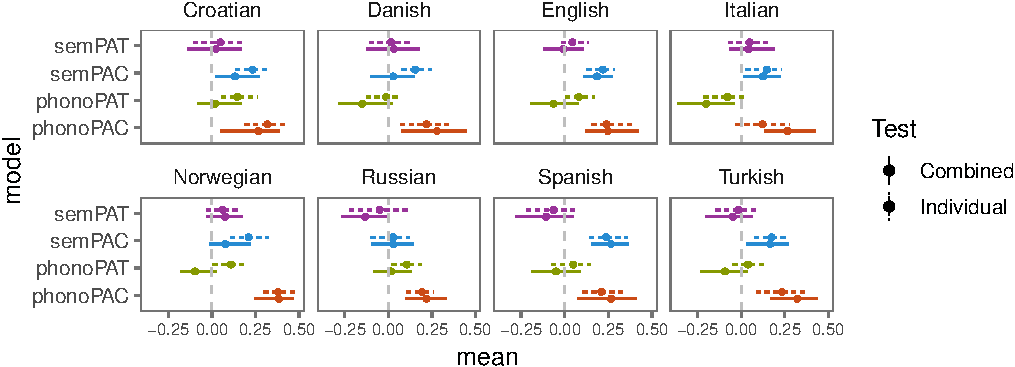
\includegraphics{figs/pred_ind_img-1} 

}

\caption{\label{fig:pred_ind}Evaluation of network growth scenarios both individually (dotted), and when combined in the same growth model (solid). Each dot represents the mean of the posterior distribution of the corresponding growth parameter, with ranges representing 95\% credible intervals (computed using the highest density intervals). Positive values mean that learning proceeds according to the predictions of the growth scenario. Negative values mean that learning proceeds in opposition to the predictions of the growth scenario.}\label{fig:pred_ind_img}
\end{figure*}
\end{CodeChunk}

\subsection{Network growth models}\label{network-growth-models}

\subsubsection{How does each growth scenario predict noun
development?}\label{how-does-each-growth-scenario-predict-noun-development}

To test the network growth scenarios, we fit different growth models to
the data. We calculated the probability that a word \(w_i\), with a
growth value \(d_i\) would enter the lexicon at a given month, using a
softmax function:

\begin{equation}
 p(w_i)= \frac{e^{\beta d_i}}{\sum_j e^{\beta d_j} }
\end{equation}

\noindent where \(\beta\) is a fitted parameter that captures the
magnitude of the relationship between network parameters and growth
(analogous to a regression coefficient). A positive value of \(\beta\)
means that words with higher growth values \(d_i\) are acquired first,
and a negative value means that words with lower growth values are
acquired first (see Figure \ref{fig:growth} for an illustration of how
growth values \(d_i\) are defined in each growth scenario). The
normalization includes all words that could be learned at that month.

We estimated the parameter \(\beta\) using a Bayesian approach. The
inference was performed using the probabilistic programming language
WebPPL (N. Goodman \& Stuhlmuller, 2014). We defined a uniform prior
over \(\beta\), and at each month, we computed the likelihood function
over words that could possibly enter the lexicon at that month, fit to
the words that have been learned at that month (using formula 1). Markov
Chain Monte Carlo sampling resulted in a posterior distribution over
\(\beta\), which we summarized in Figure \ref{fig:pred_ind}.

For the semantic networks, the results replicate Hills et al.'s finding
in English, which is that the semantic network grows by PAC, not by PAT.
Moreover, this finding holds in seven of the eight languages we
examined.\footnote{One could imagine that the fact of using English free association norms cross-linguistically would decrease the effect of non-English semantic networks because of possible cultural differences. However, our findings do not support this assumption as the effects were generally similar in magnitude cross-linguistically.}
The PAC model also fits better than PAT for phonological networks. We
note however that PAT, though weaker, fares better for the phonological
networks (where it predicts part of the growth process in some languages
such as Croatian, English, Norwegian and Russian) than it does for the
semantic networks (where it is rather universally unpredictive).

\subsubsection{What is the relative contribution of each growth
model?}\label{what-is-the-relative-contribution-of-each-growth-model}

Above we evaluated the network growth scenarios individually. As a next
step, we analyzed their relative contribution to the learning process.
This was done through adding more fitted parameters to the model, that
is, by substituting \(\beta d_i\) in formula (1) with:
\[\beta_{1} d_{i, 1} + \beta_{2} d_{i, 2} + \beta_{3} d_{i, 3} + \beta_{4} d_{i, 4}\]
where the indices represent the 4 networks: semPAT, semPAC, phonoPAT and
PhonoPAC. Using the same fitting technique, we obtained the values shown
in Figure \ref{fig:pred_ind}. PAC dominates the learning. Both
phonological and semantic networks contribute to lexical growth, but the
phonological network appears to be stronger and more consistent across
languages. In summary, the findings show that both semantic and
phonological networks contribute to the learning process, and that they
both grow primarily by PAC, relying on the external connectivity in the
learning environment, rather than the internal connectivity in the
acquired lexicon.

\begin{CodeChunk}
\begin{figure*}[h]

{\centering 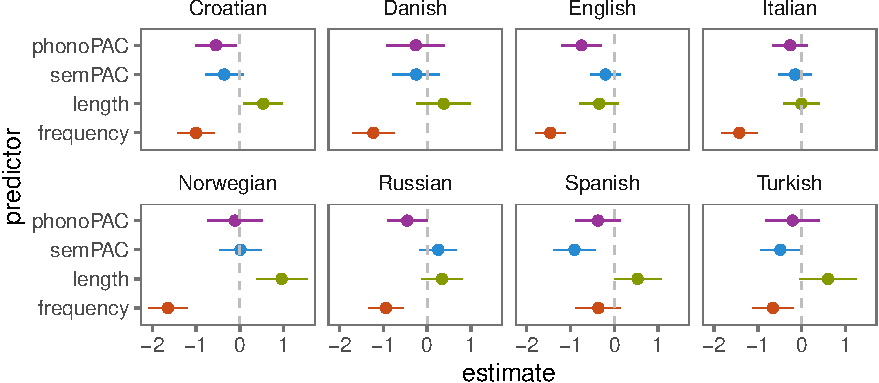
\includegraphics{figs/regressions_img-1} 

}

\caption{\label{fig:regressions_img}Estimates of predictor coefficients by language, with ranges indicating 95\% confidence intervals. Positive values indicate a positive relationship (e.g. longer words tend to have a higher AoA), while negative values indicate a negative relationship (e.g. words with higher frequency tend to have a lower AoA).}\label{fig:regressions_img}
\end{figure*}
\end{CodeChunk}

\subsection{Comparison to other predictors of age of
acquisition}\label{comparison-to-other-predictors-of-age-of-acquisition}

We saw that the way semantic and phonological information is structured
in the learning environment (i.e., PAC) contributes to noun learning
across languages. However, we know that other factors influence learning
as well (e.g., Braginsky et al., 2016). Next we investigated how
semantic and phonological connectivity interact with two other factors.
The first one is word frequency, a well studied factor shown to predict
the age of acquisition in a reliable fashion (e.g. J. C. Goodman et al.,
2008). The second factor is word length, which correlates with
phonological connectivity.

Since PAT was uninformative, we dropped it from this analysis, keeping
only PAC. This simplified the model because we no longer needed to fit
growth
month-by-month.\footnote{This was a requirement only for PAT where the words' utilities varied from month to month, depending on how connectivity changed in the growing internal network.}
A more direct way to assess and compare the contribution of PAC in
relation to other word-level factors is through conducting linear
regressions, where connectivity in the learning environment, frequency
and length predict the age of acquisition.

We used the frequency estimates from Braginsky et al. (2016) where
unigram counts were derived based on CHILDES corpora in each
language.\footnote{Note that these frequency counts are based on transcripts from independent sets of children and represent a general estimate of environmental frequency across children.}
For each word, counts included words that shared the same stem (e.g.,
``cats'' counts as ``cat''), or words that were synonymous (e.g.
``father'' counts as ``daddy''). For word length, we counted the number
of phonemes in our generated IPA transcription.

We conducted two analyses. We fit a linear regression for each language,
and we fit a linear mixed-effect model to all the data pooled across
languages, with language as a random effect. Figure
\ref{fig:regressions_img} shows the coefficient estimate for each
predictor in each language, and Figure \ref{fig:regressions_all_img}
shows the coefficient estimates for all languages combined (all
predictors were centered and scaled). The findings were as follows.
Overall, frequency is the largest and most consistent predictor of age
of acquisition, replicating results for nouns across a variety of
analyses (Braginsky et al., 2016; J. C. Goodman et al., 2008; B. C. Roy,
Frank, DeCamp, Miller, \& Roy, 2015). Word length predicts learning in
some languages such as Croatian and Norwegian, but not in others
(including English). It remains, however, a significant predictor in the
global model. As for the factors of interest, i.e., semantic and
phonological connectivity, we also found cross-linguistic differences.
Phonological connectivity contributes to learning in languages such as
Croatian, English and Russian, whereas semantic connectivity contributes
to learning in Turkish, Spanish and to some extent in Croatian, but not
in
English.\footnote{Semantic connectivity does not explain variance in English data beyond that explained by phonological connectivity, frequency and length. This contrasts with the original finding in Hills et al. 2009. However, in this previous study, semantic connectivity was not tested in a model that included frequency, length and phonological connectivity as covariates. Another important difference is the number of words tested: Our study uses a larger set of nouns.}
Despite these cross-linguistic differences, both phonological and
semantic connectivity are significant predictors in the combined model.

\section{Discussion}\label{discussion}

The present study provided a comprehensive analysis of how lexical
connectivity influences the age of acquisition of nouns in toddlers. We
compared two network growth scenarios and assessed their relative
contributions across eight languages. One scenario, PAT, described a
rich-get-richer network growth model in which the structure of the
learner's internal network determines future growth; the other, PAC,
described a model in which the external, global environmental network
structure determines learners' growth patterns. Our findings largely
replicate the results obtained by Hills et al. (2009): Semantic networks
grow by preferential acquisition, not by preferential attachment. A
novel finding is that phonological networks also grow primarily by
preferential acquisition. Moreover, both semantic and phonological
connectivity in the learning environment predict growth. These findings
generalize well across languages. When pitted against other known
predictors of age of acquisition (word frequency and length), the effect
of word connectivity shows a cross-linguistic variation, predicting
learning in some languages, but not in others. Nevertheless, this
cross-linguistic variability is to be taken with a grain of salt as it
might be exaggerated in our study by the limited and
partially-overlapping sample of nouns for each language. In fact, both
phonological and semantic connectivity are significant predictors when
data are pooled across languages.

\begin{CodeChunk}
\begin{figure}[H]

{\centering 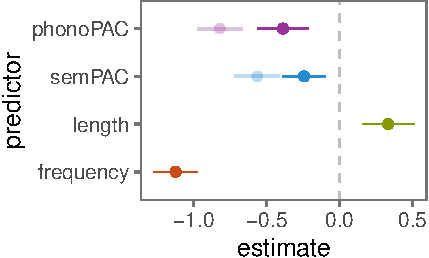
\includegraphics{figs/regressions_all_img-1} 

}

\caption{\label{fig:regressions_all_img}Estimates of predictor coefficients in the combined mixed-effect model with language as a random effect. Ranges indicate 95\% confidence intervals. Lighter points indicate estimates of PAC predictors in a model that does not include frequency and length as covariates.}\label{fig:regressions_all_img}
\end{figure}
\end{CodeChunk}

Children start by learning words that have high semantic and
phonological similarity to a variety of other words in the learning
environment, not in the child's available lexicon. This result suggests
that children are sensitive to connectivity even without having first
acquired the connected words. How can children indirectly detect highly
connected words, and why would such words be more readily learned?

In the semantic case, the networks are based on free association norms.
These associations can be (partly) derived from the patterns of
word-word co-occurrence (e.g., Griffiths, Steyvers, \& Tenenbaum, 2007),
i.e., two words are associated if they co-occur in many different
contexts. In a network structure, highly connected words would be the
words that co-occur with many other words in various contexts. Why would
such words be easier to learn? One possibility, suggested by Hills et
al. (2010), is that the referents of these words are more easily
disambiguated from other potential referents because their presence in
multiple contexts provides more cross-situational, disambiguating
statistics about their true referents (Smith \& Yu, 2008).

In the phonological case, connectivity is inherently correlated with
phonotactic probability (Vitevitch, Luce, Pisoni, \& Auer, 1999). That
is, highly connected words tend to be made of frequent sound sequences.
Even infants show a sensitivity for high frequency sound sequences in
the ambient language (Jusczyk, Luce, \& Charles-Luce, 1994). Moreover,
phonotactic probability facilitates learning and recognition (e.g.,
Storkel, 2001). In other words, children's sensitivity to local
phonotactic regularities might lead them to learn higher-probability
words more easily. This learning effect, in turn, would lead to an
observed pattern of growth that would appear to follow the PAC growth
model even though learners themselves would only be tracking local
statistics.

Finally, while validating previous results using network growth models,
our study suggests that these correlational patterns may emerge from the
operation of simpler mechanisms in both the semantic and phonological
domains. One question for future experimental work is whether such
patterns of growth can be produced in controlled behavioral experiments.

\vspace{1em}

\fbox{\parbox[b][][c]{7.3cm}{\centering All data and code for these analyses are available at\ \url{https://github.com/afourtassi/networks}}}
\vspace{1em}

\section{Acknowledgements}\label{acknowledgements}

This work was supported by a post-doctoral grant from the Fyssen
Foundation, NSF \#1528526, and NSF \#1659585.

\section{References}\label{references}

\setlength{\parindent}{-0.1in} \setlength{\leftskip}{0.125in} \noindent

\hypertarget{refs}{}
\hypertarget{ref-barabasi99}{}
Barabasi, A.-L., \& Albert, R. (1999). Emergence of scaling in random
networks. \emph{Science}, \emph{286}(5439), 509--512.

\hypertarget{ref-braginsky2016}{}
Braginsky, M., Yurovsky, D., Marchman, V. A., \& Frank, M. C. (2016).
From uh-oh to tomorrow: Predicting age of acquisition for early words
across languages. In \emph{Proceedings of the 38th Annual Conference of
the Cognitive Science Society}.

\hypertarget{ref-clauset09}{}
Clauset, A., Shalizi, C. R., \& Newman, M. E. J. (2009). Power-law
distributions in empirical data. \emph{SIAM Review}, \emph{51}(4),
661--703.

\hypertarget{ref-fenson94}{}
Fenson, L., Dale, P. S., Reznick, J. S., Bates, E., Thal, D. J.,
Pethick, S. J., \ldots{} Stiles, J. (1994). Variability in early
communicative development. \emph{Monographs of the Society for Research
in Child Development}, \emph{59}(5), i--185.

\hypertarget{ref-frank2017}{}
Frank, M. C., Braginsky, M., Yurovsky, D., \& Marchman, V. A. (2017).
Wordbank: An open repository for developmental vocabulary data.
\emph{Journal of Child Language}, \emph{44}(3), 677--694.

\hypertarget{ref-gillespie15}{}
Gillespie, C. S. (2015). Fitting heavy tailed distributions: The
poweRlaw package. \emph{Journal of Statistical Software}, \emph{64}(2),
1--16. Retrieved from \url{http://www.jstatsoft.org/v64/i02/}

\hypertarget{ref-goodman2008}{}
Goodman, J. C., Dale, P. S., \& Li, P. (2008). Does frequency count?
Parental input and the acquisition of vocabulary. \emph{Journal of Child
Language}, \emph{35}(3), 515--531.

\hypertarget{ref-dippl}{}
Goodman, N., \& Stuhlmuller, A. (2014). The Design and Implementation of
Probabilistic Programming Languages. \url{http://dippl.org}.

\hypertarget{ref-griffiths07}{}
Griffiths, T. L., Steyvers, M., \& Tenenbaum, J. B. (2007). Topics in
semantic representation. \emph{Psychological Review}, \emph{114}(2),
2007.

\hypertarget{ref-hills2010}{}
Hills, T. T., Maouene, J., Riordan, B., \& Smith, L. B. (2010). The
associative structure of language: Contextual diversity in early word
learning. \emph{Journal of Memory and Language}, \emph{63}(3), 259--273.

\hypertarget{ref-hills2009}{}
Hills, T. T., Maouene, M., Maouene, J., Sheya, A., \& Smith, L. (2009).
Longitudinal analysis of early semantic networks: Preferential
attachment or preferential acquisition? \emph{Psychological Science},
\emph{20}(6), 729--739.

\hypertarget{ref-jusczyk1994}{}
Jusczyk, P. W., Luce, P. A., \& Charles-Luce, J. (1994). Infant's
sensitivity to phonotactic patterns in the native language.
\emph{Journal of Memory and Language}, \emph{33}(5), 630--645.

\hypertarget{ref-nelson1998}{}
Nelson, D. L., McEvoy, C. L., \& Schreiber, T. A. (1998). The University
of South Florida word association, rhyme, and word fragment norms.
Retrieved from \url{http://w3.usf.edu/FreeAssociation/}

\hypertarget{ref-roy2015}{}
Roy, B. C., Frank, M. C., DeCamp, P., Miller, M., \& Roy, D. (2015).
Predicting the birth of a spoken word. \emph{Proceedings of the National
Academy of Sciences}, \emph{112}(41), 12663--12668.

\hypertarget{ref-smith2008}{}
Smith, L., \& Yu, C. (2008). Infants rapidly learn word-referent
mappings via cross-situational statistics. \emph{Cognition},
\emph{106}(3), 1558--1568.

\hypertarget{ref-steyvers2005}{}
Steyvers, M., \& Tenenbaum, J. B. (2005). The large-scale structure of
semantic networks: Statistical analyses and a model of semantic growth.
\emph{Cognitive Science}, \emph{29}(1), 41--78.

\hypertarget{ref-storkel2001}{}
Storkel, H. L. (2001). Learning new words: Phonotactic probability in
language development. \emph{Journal of Speech, Language, and Hearing
Research}, \emph{44}(6), 1321--1337.

\hypertarget{ref-storkel2009}{}
Storkel, H. L. (2009). Developmental differences in the effects of
phonological, lexical and semantic variables on word learning by
infants. \emph{Journal of Child Language}, \emph{36}(2), 29--321.

\hypertarget{ref-vitevitch1999}{}
Vitevitch, M. S., Luce, P. A., Pisoni, D. B., \& Auer, E. T. (1999).
Phonotactics, neighborhood activation, and lexical access for spoken
words. \emph{Brain and Language}, \emph{68}(1), 306--311.

\end{document}
